%; whizzy paragraph -pdf xpdf -latex ./whizzypdfptex.sh
%; whizzy-paragraph "^\\\\begin{frame}\\|\\\\emtext"
% latex beamer presentation.
% platex, latex-beamer でコンパイルすることを想定。

%     Tokyo Debian Meeting resources
%     Copyright (C) 2012 Junichi Uekawa

%     This program is free software; you can redistribute it and/or modify
%     it under the terms of the GNU General Public License as published by
%     the Free Software Foundation; either version 2 of the License, or
%     (at your option) any later version.

%     This program is distributed in the hope that it will be useful,
%     but WITHOUT ANY WARRANTY; without even the implied warreanty of
%     MERCHANTABILITY or FITNESS FOR A PARTICULAR PURPOSE.  See the
%     GNU General Public License for more details.
%     You should have received a copy of the GNU General Public License
%     along with this program; if not, write to the Free Software
%     Foundation, Inc., 51 Franklin St, Fifth Floor, Boston, MA  02110-1301 USA

\documentclass[cjk,dvipdfmx,12pt]{beamer}
\usetheme{Tokyo}
\usepackage{monthlypresentation}

%  preview (shell-command (concat "evince " (replace-regexp-in-string "tex$" "pdf"(buffer-file-name)) "&"))
%  presentation (shell-command (concat "xpdf -fullscreen " (replace-regexp-in-string "tex$" "pdf"(buffer-file-name)) "&"))
%  presentation (shell-command (concat "evince " (replace-regexp-in-string "tex$" "pdf"(buffer-file-name)) "&"))

%http://www.naney.org/diki/dk/hyperref.html
%日本語EUC系環境の時
\AtBeginDvi{\special{pdf:tounicode EUC-UCS2}}
%シフトJIS系環境の時
%\AtBeginDvi{\special{pdf:tounicode 90ms-RKSJ-UCS2}}

\newenvironment{commandlinesmall}%
{\VerbatimEnvironment
  \begin{Sbox}\begin{minipage}{1.0\hsize}\begin{fontsize}{8}{8} \begin{BVerbatim}}%
{\end{BVerbatim}\end{fontsize}\end{minipage}\end{Sbox}
  \setlength{\fboxsep}{8pt}
% start on a new paragraph

\vspace{6pt}% skip before
\fcolorbox{dancerdarkblue}{dancerlightblue}{\TheSbox}

\vspace{6pt}% skip after
}
%end of commandlinesmall

\title{Gmail とパスワード}
%\subtitle{}
\author{yy\_y\_ja\_jp}
\date{2022-05-21}
\logo{
\includegraphics[width=8cm]{image-assets/openlogo-light.eps}}

\begin{document}

\begin{frame}
\titlepage{}
\end{frame}

% \section{Agenda}

\begin{frame}{Debian とメール}

Debianでメールを使う(特に送る)機会
\begin{itemize}
 \item キーサイン
 \item バグ報告
 \item 投票(Debian 公式開発者)
 \item ...
\end{itemize}

Webメール以外を使うこともあったりする

\end{frame}

\begin{frame}{Google 曰く ``安全性の低いアプリ''}

Gmailは最近までメールクライアントからGoogle アカウントのユーザー名とパスワードでアクセスする設定ができていた

今2022年5月現在は新たな有効化ができない

{\footnotesize\url{https://myaccount.google.com/security?hl=ja}}

\begin{center}
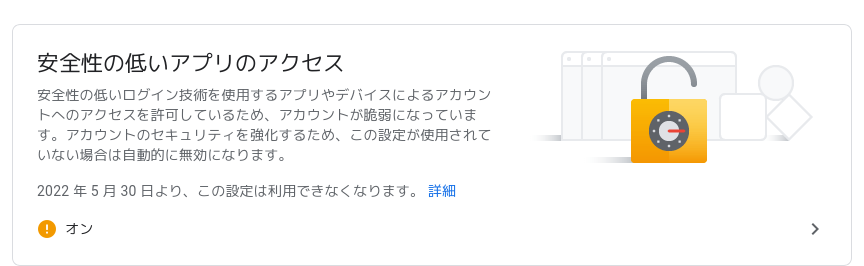
\includegraphics[width=0.9\hsize]{image202205/g-security-less.png}

(有効化済みアカウントでの表示)
\end{center}

\begin{quote}
 % 安全性の低いログイン技術を使用するアプリやデバイスによるアカウントへのアクセスを許可しているため、アカウントが脆弱になっています。アカウントのセキュリティを強化するため、この設定が使用されていない場合は自動的に無効になります。
2022 年 5 月 30 日より、この設定は利用できなくなります。
\end{quote}

\end{frame}

\begin{frame}{``安全性の低いアプリと Google アカウント''}

{\footnotesize\url{https://support.google.com/accounts/answer/6010255?hl=ja}}

\begin{center}
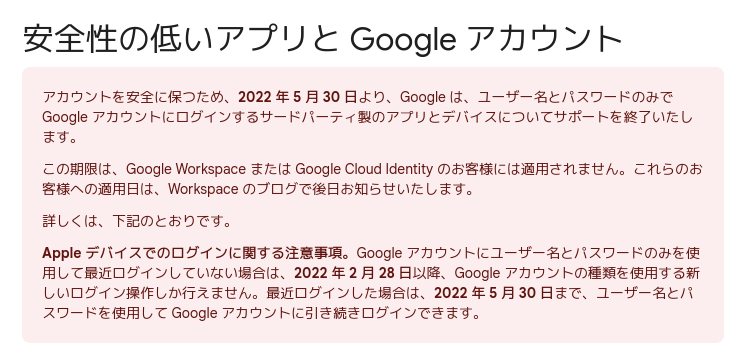
\includegraphics[width=0.8\hsize]{image202205/g-support-less.png}
\end{center}

\begin{quote}
アカウントを安全に保つため、2022 年 5 月 30 日より、Google は、ユーザー名とパスワードのみで Google アカウントにログインするサードパーティ製のアプリとデバイスについてサポートを終了いたします。
\end{quote}

\end{frame}

\begin{frame}{Google アカウント ``アプリ パスワード''}

{\footnotesize\url{https://support.google.com/accounts/answer/185833?hl=ja}}

\begin{center}
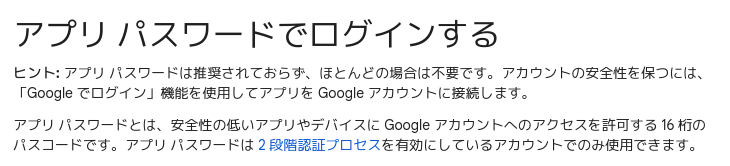
\includegraphics[width=1\hsize]{image202205/g-support-apppass.png}
\end{center}

% \begin{quote}
% ヒント: アプリ パスワードは推奨されておらず、ほとんどの場合は不要です。アカウントの安全性を保つには、「Google でログイン」機能を使用してアプリを Google アカウントに接続します。

% アプリ パスワードとは、安全性の低いアプリやデバイスに Google アカウントへのアクセスを許可する 16 桁のパスコードです。アプリ パスワードは 2 段階認証プロセスを有効にしているアカウントでのみ使用できます。
% \end{quote}

\begin{itemize}
 \item アカウントパスワードのアプリ向け代替
 \item Googleは推奨していない
 \item Googleは「Google でログイン」機能(OAuth認証)を推奨 -- メールクライアントが対応している必要がある
 \item アプリ パスワードをGoogle アカウントで使うには ``2 段階認証プロセス'' の有効化が必須

\end{itemize}

\end{frame}

\begin{frame}{``2 段階認証プロセス''}

{\footnotesize\url{https://support.google.com/accounts/answer/185839}}

\begin{center}
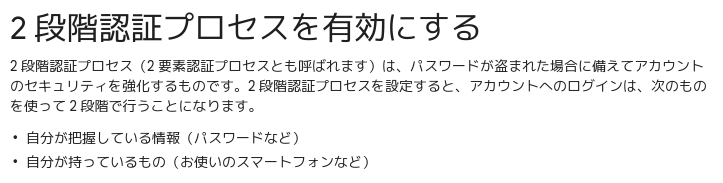
\includegraphics[width=0.9\hsize]{image202205/g-support-twostepverif.png}
\end{center}

\begin{quote}
2 段階認証プロセス(2 要素認証プロセスとも呼ばれます)は、パスワードが盗まれた場合に備えてアカウントのセキュリティを強化するものです。2 段階認証プロセスを設定すると、アカウントへのログインは、次のものを使って 2 段階で行うことになります。

\begin{itemize}
 \item     自分が把握している情報(パスワードなど)
 \item     自分が持っているもの(お使いのスマートフォンなど)
\end{itemize}
\end{quote}

\end{frame}

\begin{frame}{Google アカウント 2 段階認証プロセス}

{\footnotesize\url{https://myaccount.google.com/security?hl=ja}}

\begin{center}
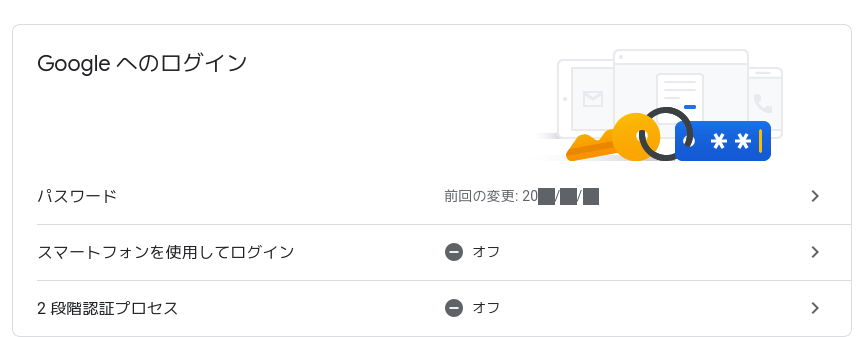
\includegraphics[width=0.9\hsize]{image202205/g-security-signinopts-0.png}
\end{center}

\begin{quote}
\end{quote}

⇒ 2 段階認証プロセスを有効化してみる

\end{frame}

\begin{frame}{Google アカウント 2 段階認証プロセス}

{\footnotesize\url{https://myaccount.google.com/signinoptions/two-step-verification}}

\begin{center}
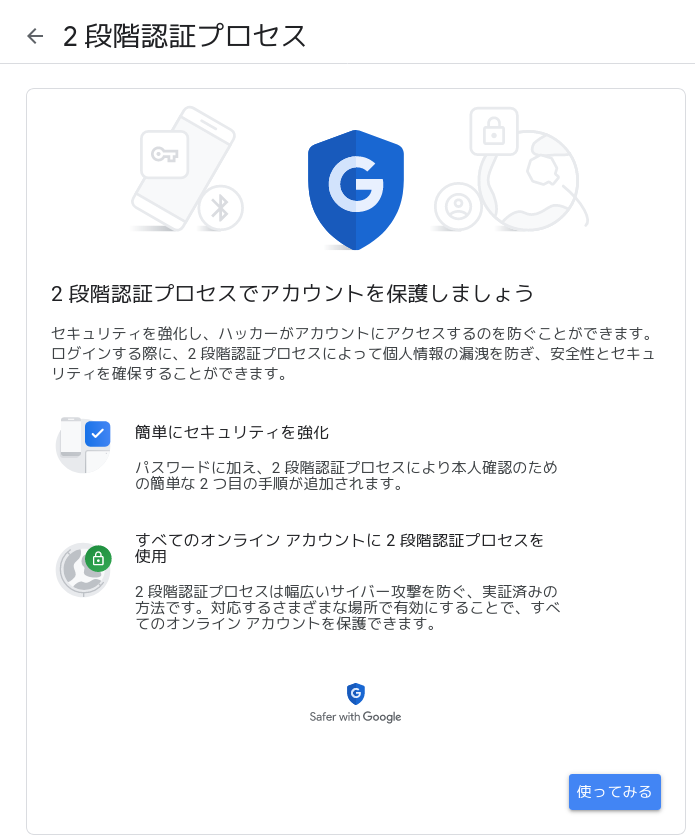
\includegraphics[width=0.5\hsize]{image202205/g-signinopt-twostepverif-welcome.png}
\end{center}

\begin{quote}
\end{quote}

\end{frame}

\begin{frame}{Google アカウント 2 段階認証プロセス}

{\footnotesize\url{https://myaccount.google.com/signinoptions/two-step-verification}}

\begin{center}
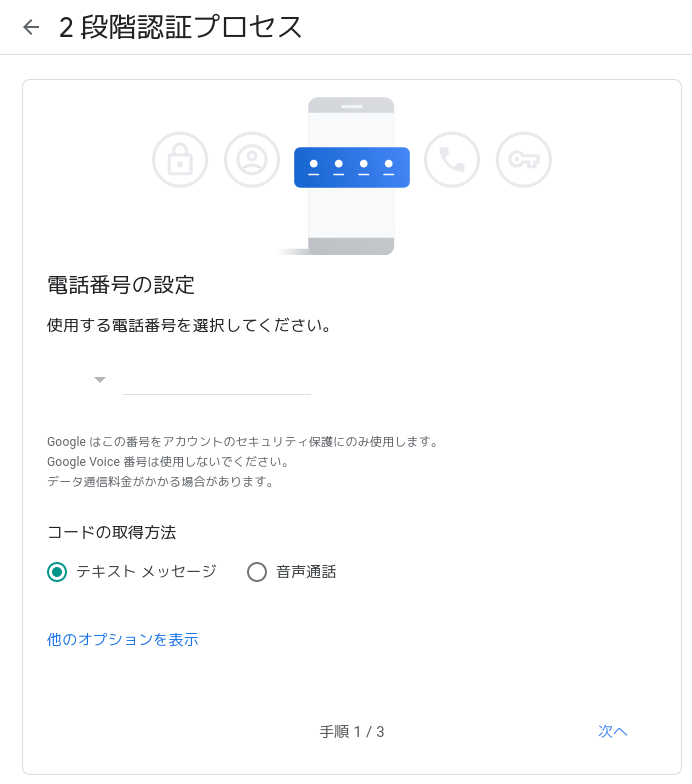
\includegraphics[width=0.45\hsize]{image202205/g-signinopt-twostepverif-enroll-1-0.png}
\end{center}

電話がデフォルトらしい

\end{frame}

\begin{frame}{Google アカウント 2 段階認証プロセス}

{\footnotesize\url{https://myaccount.google.com/signinoptions/two-step-verification}}

\begin{center}
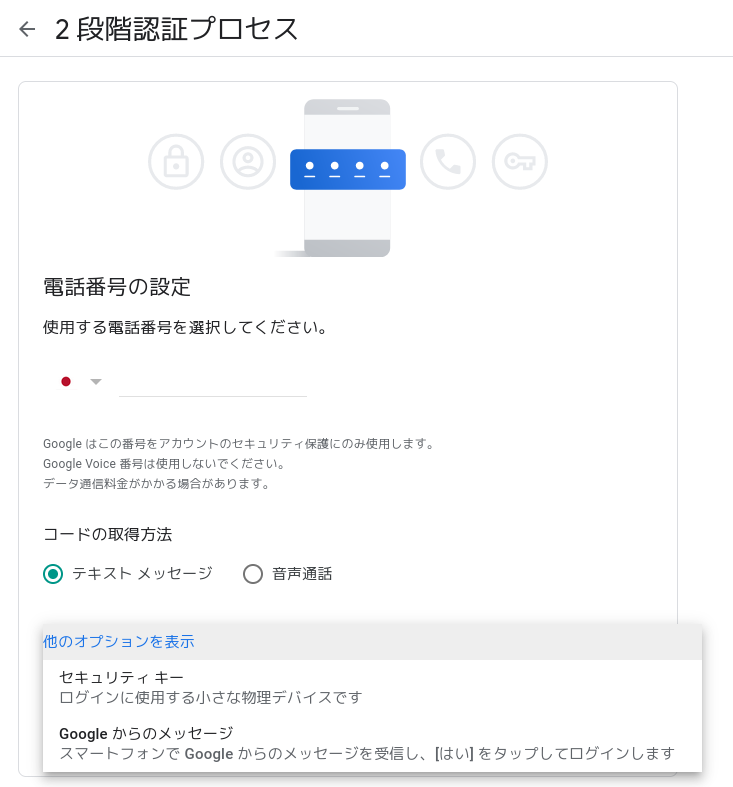
\includegraphics[width=0.45\hsize]{image202205/g-signinopt-twostepverif-enroll-1-1.png}
\end{center}

\begin{itemize}
 \item 電話
 \item セキュリティ キー -- ハードウェアキー
 \item ``Google からのメッセージ'' -- スマートフォン(≒電話)
\end{itemize}

\end{frame}

\begin{frame}{Google アカウント 2 段階認証プロセス}

{\footnotesize\url{https://myaccount.google.com/signinoptions/two-step-verification}}

\begin{center}
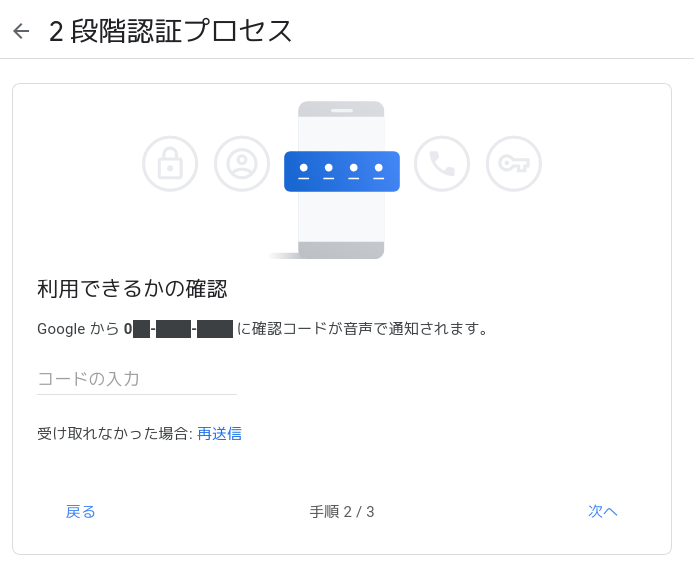
\includegraphics[width=0.5\hsize]{image202205/g-signinopt-twostepverif-enroll-2.png}
\end{center}

\begin{quote}
\end{quote}

\end{frame}

\begin{frame}{Google アカウント 2 段階認証プロセス}

{\footnotesize\url{https://myaccount.google.com/signinoptions/two-step-verification}}

\begin{center}
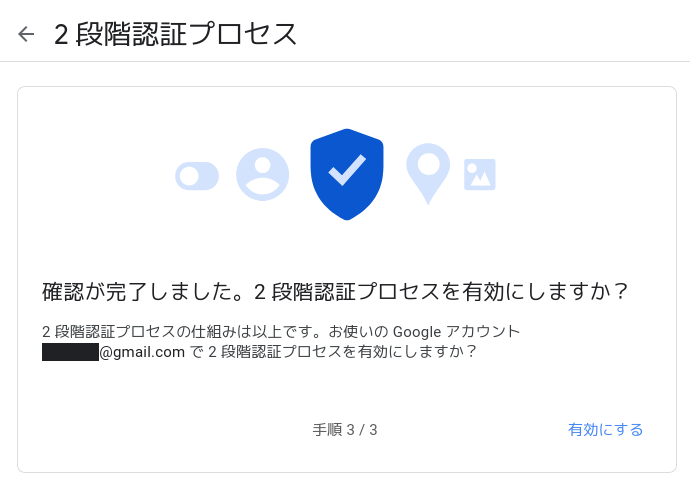
\includegraphics[width=0.5\hsize]{image202205/g-signinopt-twostepverif-enroll-3.png}
\end{center}

\begin{quote}
\end{quote}

\end{frame}

\begin{frame}{Google アカウント 2 段階認証プロセス}

{\footnotesize\url{https://myaccount.google.com/signinoptions/two-step-verification}}

\begin{center}
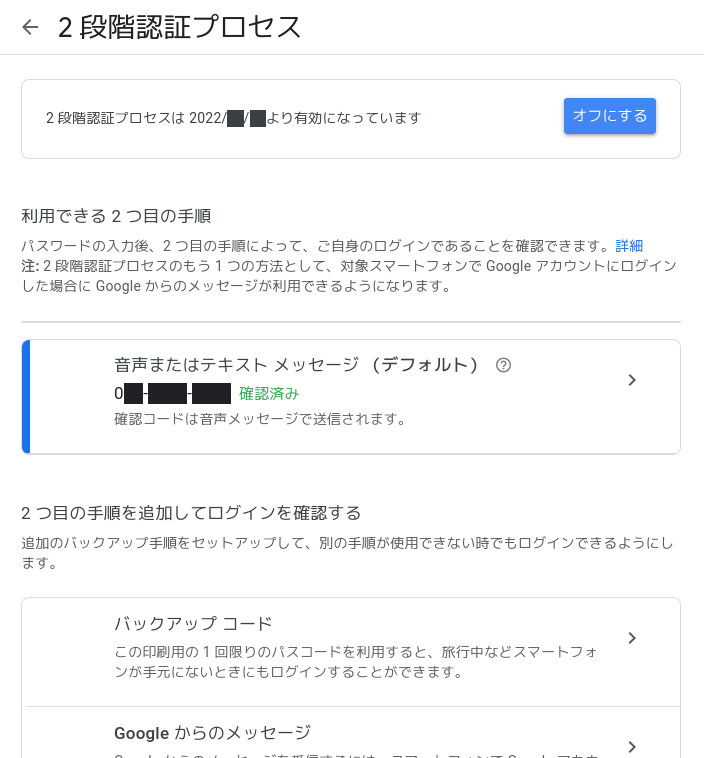
\includegraphics[width=0.5\hsize]{image202205/g-signinopt-twostepverif-0-0.png}
\end{center}

\begin{quote}
\end{quote}

\end{frame}

\begin{frame}{Google アカウント 2 段階認証プロセス}

{\footnotesize\url{https://myaccount.google.com/security?hl=ja}}

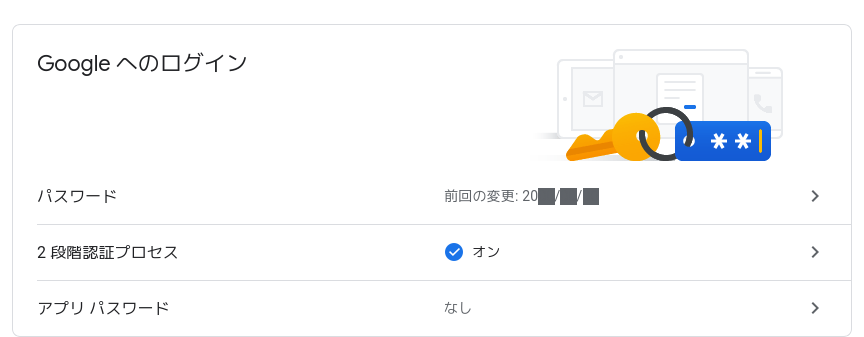
\includegraphics[width=0.9\hsize]{image202205/g-security-signinopts-1.png}

\begin{quote}
\end{quote}

⇒ 2 段階認証プロセスを有効化して選べるようになったアプリ パスワードを使ってみる

\end{frame}

\begin{frame}{Google アカウント アプリ パスワード}

{\footnotesize\url{https://myaccount.google.com/apppasswords}}

\begin{center}
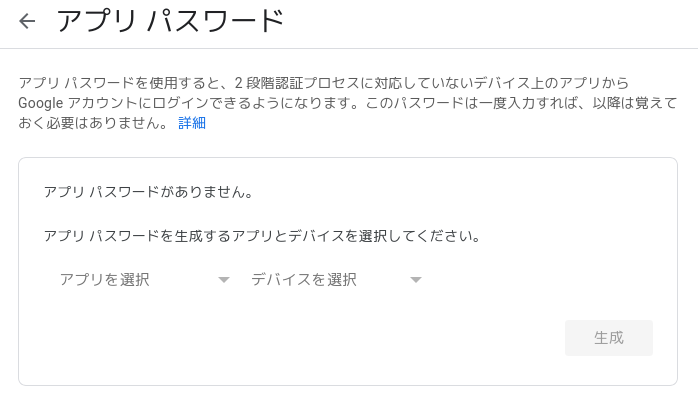
\includegraphics[width=0.8\hsize]{image202205/g-apppass-0-0.png}
\end{center}

\begin{quote}
% アプリ パスワードを使用すると、2 段階認証プロセスに対応していないデバイス上のアプリから Google アカウントにログインできるようになります。
このパスワードは一度入力すれば、以降は覚えておく必要はありません。
\end{quote}

\end{frame}

\begin{frame}{Google アカウント アプリ パスワード}

{\footnotesize\url{https://myaccount.google.com/apppasswords}}

\begin{center}
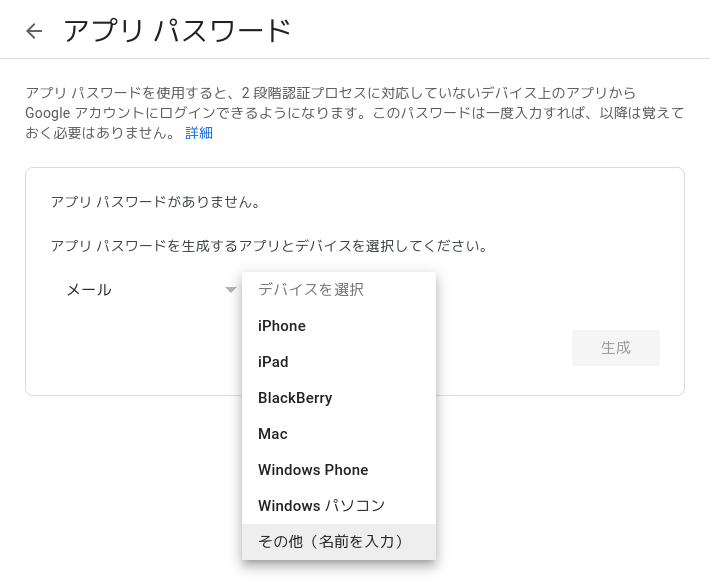
\includegraphics[width=0.8\hsize]{image202205/g-apppass-0-1.png}
\end{center}

\begin{quote}
\end{quote}

\end{frame}

\begin{frame}{Google アカウント アプリ パスワード}

{\footnotesize\url{https://myaccount.google.com/apppasswords}}

\begin{center}
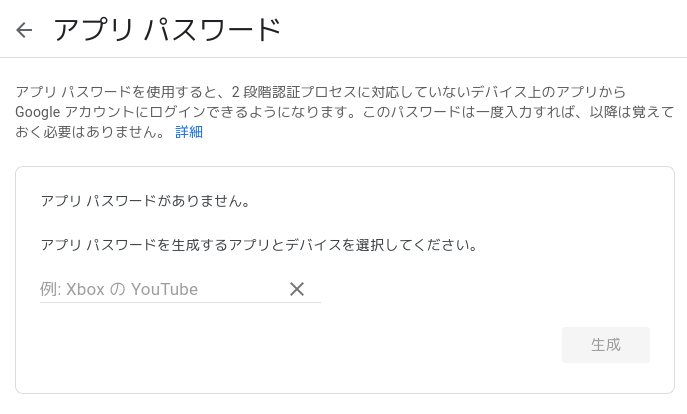
\includegraphics[width=0.8\hsize]{image202205/g-apppass-0-2.png}
\end{center}

\begin{quote}
\end{quote}

\end{frame}

\begin{frame}{Google アカウント アプリ パスワード}

{\footnotesize\url{https://myaccount.google.com/apppasswords}}

\begin{center}
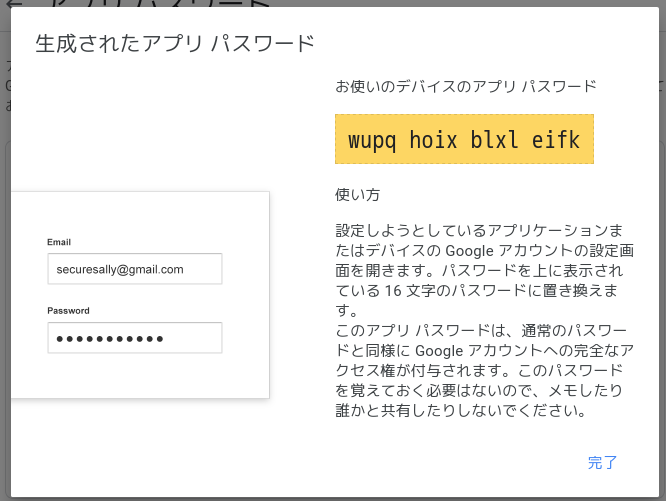
\includegraphics[width=0.65\hsize]{image202205/g-apppass-1.png}
\end{center}

⇒ このアプリ パスワードをメールクライアントでアカウントパスワードの代わりに保存して使う

今のところWebでGoogleアカウントにログインするとき2段階認証になる以外の使い勝手は基本的に変わらないはず

\end{frame}

\begin{frame}{Google アカウント アプリ パスワード}

{\footnotesize\url{https://myaccount.google.com/apppasswords}}

\begin{center}
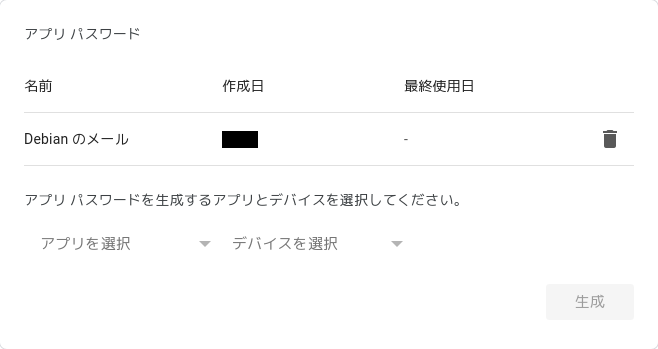
\includegraphics[width=0.8\hsize]{image202205/g-apppass-2.png}
\end{center}

⇒ 保存したはずだということでもう見られない

\end{frame}

\begin{frame}{Google アカウント 2 段階認証プロセス}

{\footnotesize\url{https://myaccount.google.com/signinoptions/two-step-verification}}

\begin{center}
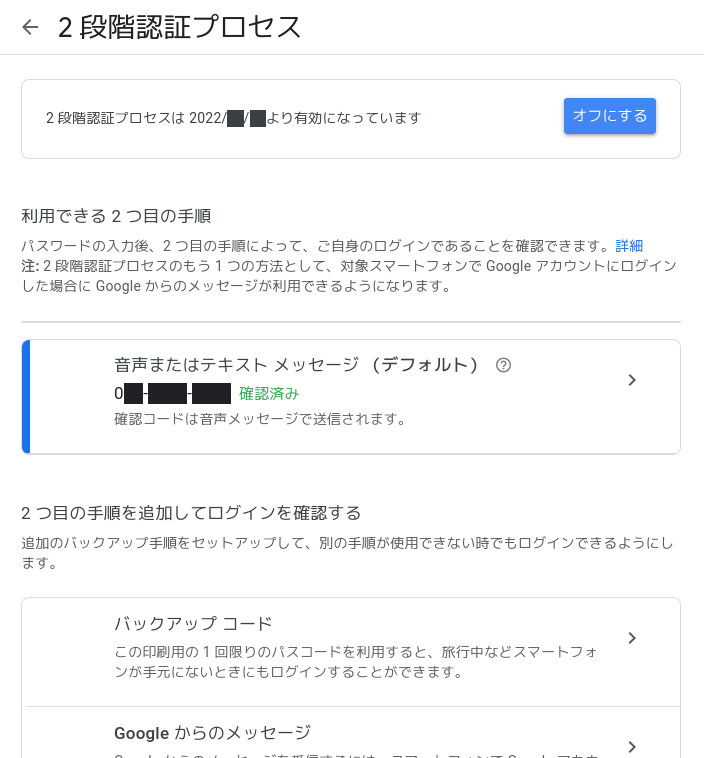
\includegraphics[width=0.5\hsize]{image202205/g-signinopt-twostepverif-0-0.png}
\end{center}

\begin{quote}
\end{quote}

\end{frame}

\begin{frame}{Google アカウント 2 段階認証プロセス}

{\footnotesize\url{https://myaccount.google.com/signinoptions/two-step-verification}}

\begin{center}
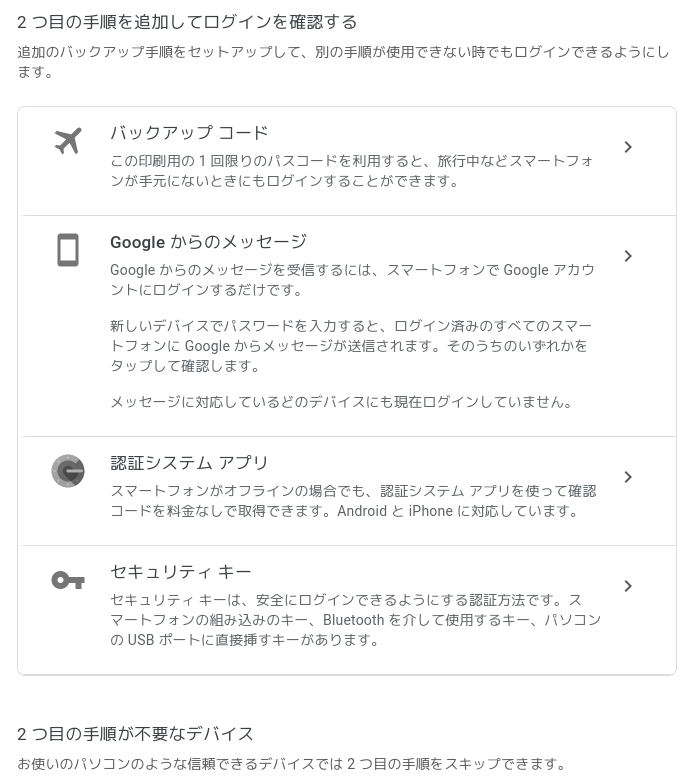
\includegraphics[width=0.5\hsize]{image202205/g-signinopt-twostepverif-0-1.png}
\end{center}

電話・ハードウェアキー以外の選択肢が増える

\begin{quote}
\end{quote}

\end{frame}

\begin{frame}{Google アカウント ``認証システム アプリ''}

{\footnotesize\url{https://myaccount.google.com/signinoptions/two-step-verification}}

\begin{center}
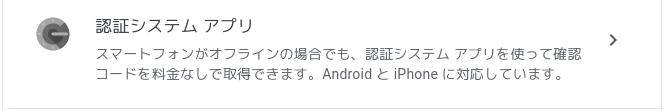
\includegraphics[width=0.9\hsize]{image202205/g-signinopt-twostepverif-0-2.png}
\end{center}

\begin{quote}
スマートフォンがオフラインの場合でも、認証システム アプリを使って確認コードを料金なしで取得できます。Android と iPhone に対応しています。
\end{quote}

⇒ 実はスマートフォンでなくてもよいのでやってみる

\end{frame}

\begin{frame}{Google アカウント ``認証システム アプリ''}

{\footnotesize\url{https://myaccount.google.com/two-step-verification/authenticator}}

\begin{center}
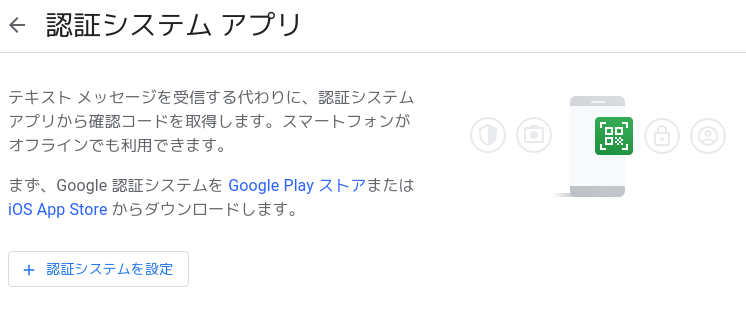
\includegraphics[width=0.9\hsize]{image202205/g-twostepverif-authenticator-0.png}
\end{center}

\begin{quote}
まず、Google 認証システムを Google Play ストアまたは iOS App Store からダウンロードします。
\end{quote}

``Google 認証システム (Google Authenticator)'' アプリのことを指してはいる

\end{frame}

\begin{frame}{Google アカウント 認証システム アプリの設定}

{\footnotesize\url{https://myaccount.google.com/two-step-verification/authenticator}}

\begin{center}
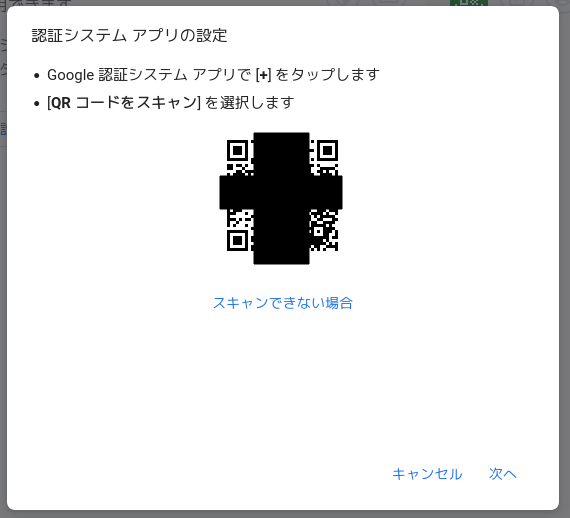
\includegraphics[width=0.3\hsize]{image202205/g-twostepverif-authenticator-1-1.png}
\end{center}

\begin{quote}
\begin{itemize}
 \item Google 認証システム アプリで [+] をタップします
 \item {[QR コードをスキャン] を選択します}
\end{itemize}
\end{quote}

⇒ などと書いてあるがとりあえず無視してQRコード画像を安全な場所に保存しておく

⇒ ``スキャンできない場合'' も見てみる

\end{frame}

\begin{frame}[containsverbatim]{Google アカウント 認証システム アプリの設定}

{\footnotesize\url{https://myaccount.google.com/two-step-verification/authenticator}}

\begin{center}
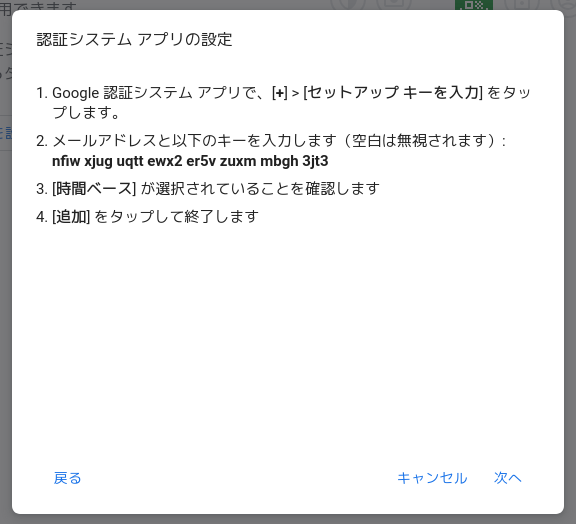
\includegraphics[width=0.3\hsize]{image202205/g-twostepverif-authenticator-1-2.png}
\end{center}

\begin{quote}
\begin{enumerate}
 \item 
    Google 認証システム アプリで、[+] $>$ [セットアップ キーを入力] をタップします。
 \item 
    メールアドレスと以下のキーを入力します(空白は無視されます):\\
    {\footnotesize\verb|nfiw xjug uqtt ewx2 er5v zuxm mbgh 3jt3|}
 \item 
    {[時間ベース] が選択されていることを確認します}
 \item 
    {[追加] をタップして終了します}
\end{enumerate}
\end{quote}

\end{frame}

\begin{frame}[containsverbatim]{認証システム アプリの設定 -- QRコード}

\begin{commandlinesmall}
# apt install zbar-tools
# 
$ zbarimg index.png
QR-Code:otpauth://totp/Google%3A**********%40gmail.com?secret=nfiwxjuguqtt
ewx2er5vzuxmmbgh3jt3&issuer=Google
scanned 1 barcode symbols from 1 images in 0.01 seconds
$ 
$ zbarimg -q --raw index.png | sed 's/.*secret=\([[:alnum:]]*\).*/\1/'
nfiwxjuguqttewx2er5vzuxmmbgh3jt3
$ 
\end{commandlinesmall}
認証システム アプリに必要な鍵情報がURI形式で書かれている 標準化はされてないようだが他サービスも概ね``Google 認証システム''アプリに合わせている模様
\begin{itemize}
 \item {\footnotesize\verb|totp|} -- ``時間ベース'' (Time-based One-Time Password)
 \item {\footnotesize\verb|**********@gmail.com|} -- ``メールアドレス'' アカウント名(QRコードには手入力せずとも含まれている)
 \item {\footnotesize\verb|nfiwxjuguqttewx2er5vzuxmmbgh3jt3|} -- ``セットアップ キー'' 秘密鍵(base32 エンコード)
 \item {\footnotesize\verb|Google|} -- サービス名
\end{itemize}

\end{frame}

\begin{frame}{Google アカウント 認証システム アプリの設定}

{\footnotesize\url{https://myaccount.google.com/two-step-verification/authenticator}}

\begin{center}
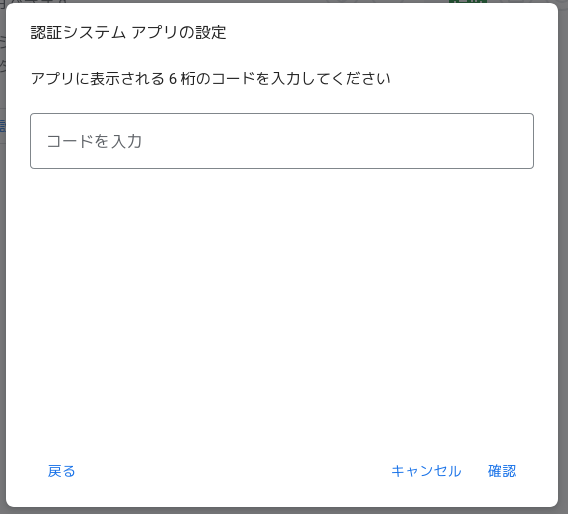
\includegraphics[width=0.5\hsize]{image202205/g-twostepverif-authenticator-1-3.png}
\end{center}

\begin{quote}
アプリに表示される 6 桁のコードを入力してください
\end{quote}

\end{frame}

\begin{frame}[containsverbatim]{``認証システム アプリ''}

``時間ベース'' -- TOTP (Time-based One-Time Password) を実装しているソフトウェアなら互換性がある

コード表示に秘密鍵は必要だがサービス名やアカウント名は不要

\begin{commandlinesmall}
# apt install oathtool
# 
$ zbarimg -q --raw index.png | sed 's/.*secret=\([[:alnum:]]*\).*/\1/' | 
oathtool --totp --base32 -
789613
$ zbarimg -q --raw index.png | sed 's/.*secret=\([[:alnum:]]*\).*/\1/' | 
oathtool -w 10 --totp --base32 -
789613
067410
818083
260090
232806
105748
078883
190238
164080
397309
870025
$ 
\end{commandlinesmall}

\end{frame}

\begin{frame}{Google アカウント 認証システム アプリの設定}

{\footnotesize\url{https://myaccount.google.com/two-step-verification/authenticator}}

\begin{center}
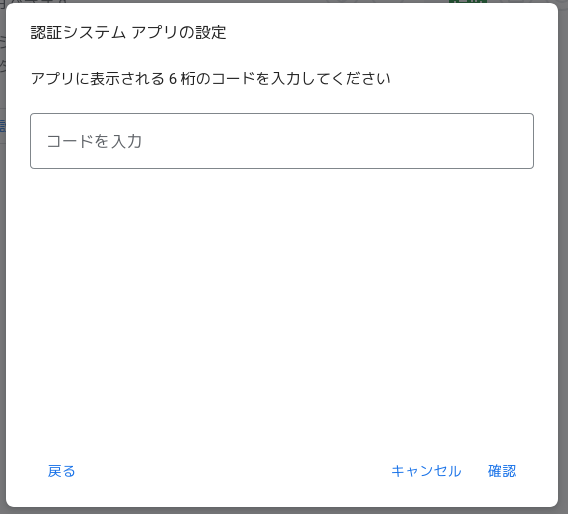
\includegraphics[width=0.5\hsize]{image202205/g-twostepverif-authenticator-1-3.png}
\end{center}

\begin{quote}
アプリに表示される 6 桁のコードを入力してください
\end{quote}

⇒ (互換)アプリのコードを入力

\end{frame}

\begin{frame}{Google アカウント 認証システム アプリ}

{\footnotesize\url{https://myaccount.google.com/two-step-verification/authenticator}}

\begin{center}
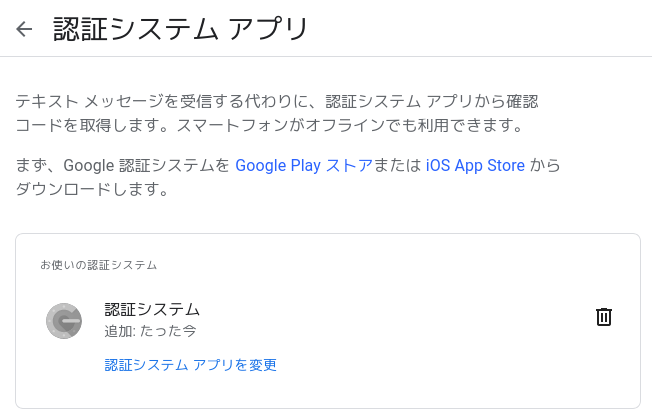
\includegraphics[width=0.8\hsize]{image202205/g-twostepverif-authenticator-2.png}
\end{center}

\begin{quote}
% 認証システム アプリ
\end{quote}

\end{frame}

\begin{frame}{Google アカウント 2 段階認証プロセス}

{\footnotesize\url{https://myaccount.google.com/signinoptions/two-step-verification}}

\begin{center}
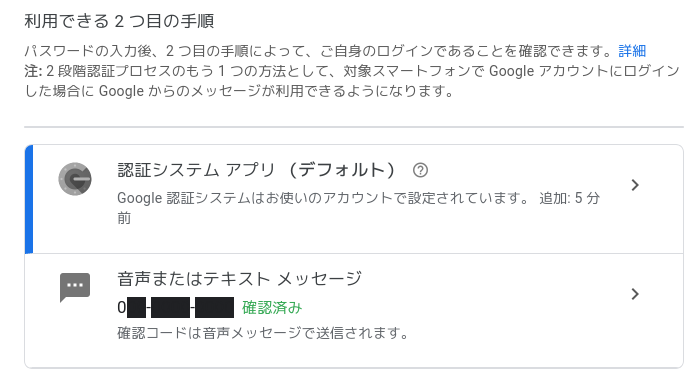
\includegraphics[width=0.7\hsize]{image202205/g-signinopt-twostepverif-2.png}
\end{center}

\begin{quote}
\end{quote}

⇒ 電話が外せる

\end{frame}

\begin{frame}{認証システム アプリの鍵情報の管理}

\begin{itemize}
 \item 認証システム アプリに管理してもらう\\
⇒ アカウント名・サービス名も保存される(アプリによる)
 \item QRコード画像の保存\\
⇒ アカウント名・サービス名も保存される
 \item セットアップ キー自体をパスワードマネージャ等に保存
\end{itemize}

\end{frame}

\begin{frame}{まとめ}

\begin{itemize}
 \item メールクライアントでGmailのアカウントパスワードが使えなくなる
 \item Google推奨のOAuth認証を使うにはメールクライアントの対応が必須
 \item 代替のアプリパスワード(Google非推奨)を使うには 2 段階認証プロセスが必須
 \item 認証システム アプリ(Authenticator)互換ソフトウェアを使えば 2 段階認証プロセスをDebian PCでもできる
 \item 認証システム アプリの鍵情報の管理に気をつける
\end{itemize}

\end{frame}

\end{document}

;;; Local Variables: ***
;;; outline-regexp: "\\([ 	]*\\\\\\(documentstyle\\|documentclass\\|emtext\\|section\\|begin{frame}\\)\\*?[ 	]*[[{]\\|[]+\\)" ***
;;; End: ***
